\chapter{Ejemplo de ligaduras no holónomas}

	
\begin{tikzpicture}
	\fill [left color=red!50, right color=teal!50] (0,0) rectangle (6.5,.1);
	\fill [left color=teal!50, right color=blue!50] (6.5,0) rectangle (11.5,.1);
	\end{tikzpicture}



\vspace{10mm}
\begin{adjustwidth}{50pt}{50pt}
\begin{ejemplo}
Ejemplo de ligaduras no holónomas: cuerpo sin fricción sobre plano inclinado sin fricción.
\end{ejemplo}
\end{adjustwidth}
\vspace{5mm}

\section{Ejemplo de ligaduras no holónomas}

\begin{example}
	
\begin{multicols}{2}
\begin{figure}[H]
	\centering
	\includegraphics[width=.45\textwidth]{imagenes/img10-01.png}
\end{figure}	
$\,$

Una cuña de masa $M$ y pendiente $\theta$ se puede desplazar a lo largo del eje $x$. En su plano inclinado se encuentra otra masa $m$, que se puede desplazar por la pendiente. Ambas masas se desplazan \emph{sin rozamiento} ($M$ en el plano horizontal y $m$ en el plano inclinado de la cuña).
\end{multicols}
\end{example}

\normalsize{Supongamos}, en un principio, que ambas masas evolucionan libremente. Más tarde impondremos la restricción de que $m$ lo haga sobre el plano inclinado de $M$ (ligadura).

El lagrangiano del sistema será:

\begin{equation}
L \ = \ \ \ \dfrac M 2 \dot X^2 \ \ \ + \ \ \  \dfrac m 2 (\dot x^2 + \dot y^2) \ - \  mgy  \qquad \qquad \textcolor{gris}{(q_1=X;\ q_2=x; \ q_3=y)}
\end{equation}

Escribamos las ecuaciones de Euler-Lagrange correspondientes a este lagranginao, más tarde las completaremos al imponer las ligaduras del problema.
\begin{equation}
\label{T10EELsinL}
\displaystyle
\begin{cases} 
\ \displaystyle \dv{t} \left(\pdv{L}{\dot X}\right) - \pdv{L}{X} = \framebox{\textcolor{white}{lig}} \\ 
\ \displaystyle \dv{t} \left(\pdv{L}{\dot x}\right) - \pdv{L}{x} \ = \framebox{\textcolor{white}{lig}} \\ 
\ \displaystyle \dv{t} \left(\pdv{L}{\dot y}\right) - \pdv{L}{y} \ = \framebox{\textcolor{white}{lig}}
\end{cases}
\to \
\begin{cases}
\ \displaystyle \dv{t}(M\dot X)-0 \ =	\framebox{\textcolor{white}{lig}} \\
\ \displaystyle \dv{t}(M\dot x)-0 \ \ \ =	\framebox{\textcolor{white}{lig}} \\
\ \displaystyle \dv{t}(M\dot y)+mg=	\framebox{\textcolor{white}{lig}} 
\end{cases}
\to \
\begin{cases}
\ M \ddot X &= \framebox{\textcolor{white}{lig}} \\
\ m \ddot x	 &= \framebox{\textcolor{white}{lig}} \\
\ m\ddot y + mg &= \framebox{\textcolor{white}{lig}}
\end{cases}
\end{equation}

En las zona $\ \framebox{\textcolor{white}{lig}} \ $ es donde aparecerán los \emph{multiplicadores de Lagrange} correspondientes a las ligaduras del problema.

Para introducir las ligaduras del problema vamos a crear dos variables auxiliares momentáneas $\textcolor{teal}{c}$ y $\textcolor{teal}{b}$ (ver figura del ejemplo) que nos facilitarán el trabajo. ($\textcolor{teal}{c}$ es la altura de cuña y $\textcolor{teal}{b}$ la distancia qua ha bajado en el plano inclinado la masa $m$).


$\begin{cases}
\ x=X+b\cos \theta \\ \ y=c-b\sin \theta	
\end{cases} \to \textcolor{gris}{(2^a \ ec)} \ \ \ b=\dfrac {y-c}{-\sin \theta} \ \to \ \textcolor{gris}{(1^a \ ec)} \ \ \ x=X-\dfrac{y-c}{\sin \theta} \cos \theta$

Derivando esta última expresión, $\quad \dot x = \dot X -\dfrac{\cos \theta}{\sin \theta} \ \dot y \qquad \textcolor{gris}{(c=cte;\ \dot c=0)}$

Multiplicando por $\sin \theta$ y ordenando esta expresión,

\begin{equation}
\label{T10ligadura}
\subrayado{\boxed{ \ \boldsymbol{ \sin \theta \ \dot X \ - \ \sin \theta \ \dot x \ - \ \cos \theta \ \dot y \ = \ 0 } \ }	}
\end{equation}

que es nuestra relación de \textbf{ligadura no holónoma}. Identificando con
la definición: $\ a_{11}q_1+a_{12}q_2+a_{13}q_3=a_{10}$, determinamos que, en nuestro caso,

\begin{equation}
\boldsymbol{ a_{11} = \sin \theta;\ \ a_{12}=-\sin \theta;\ \ a_{13}=-\cos \theta;\ \ a_{10}=0 }
\end{equation}
Y ahora volveremos con las ecuaciones de Euler-Lagrange.

\vspace{10mm}
\underline{Inciso}: $\quad$ \rule{150pt}{0.1pt} $\quad$ Teoría.
\vspace{3mm}
\begin{ejemplo}
\begin{myblock}{Ecuaciones de Euler-Lagrange para el caso de ligaduras no holónomas.}
\vspace{3mm}
\begin{large}
\begin{equation}
\boldsymbol{
\dv{t} \left( \pdv{L}{\dot q_j}\right) - \pdv{L}{q_j} \ = \ \sum_{k=1}^p \lambda_k \ a_{kj}
}
\end{equation}
\end{large}
%\vspace{2mm} 
\begin{center}\textcolor{gris}{$p$ es el número de ligaduras y $j$ el de coordenadas generalizadas}\end{center}	
\end{myblock}
\end{ejemplo}
\vspace{-5mm}
\begin{flushright}
\rule{300pt}{0.1pt}	
\end{flushright} 
\vspace{5mm}

En nuestro caso solo tenemos una ligadura (ec. \ref{T10ligadura}):

\begin{equation}
\label{T10multiplicadores}	
\quad \displaystyle 
\boxed{ \ \boldsymbol{
\dv{t} \left( \pdv{L}{\dot q_j}\right) - \pdv{L}{q_j} \ = \  \lambda \ a_j
} \ }
\end{equation}

Retomamos nuestras ecuaciones de Euler-Lagrange, ec. \ref{T10EELsinL}, y vamos a imponer nuestras ligadura (ec. \ref{T10ligadura})  con los multiplicadores de Lagrange (ec \ref{T10multiplicadores}).


\begin{equation}
\label{T10EL}
\begin{cases}
\ M \ddot X &= \textcolor{gris}{\lambda a_{11}=}\ \ \ \lambda \sin \theta \\
\ m \ddot x	&= \textcolor{gris}{\lambda a_{12}=}-\lambda \sin \theta \\
\ m \ddot y - mg &= \textcolor{gris}{\lambda a_{13}=} - \lambda \cos \theta
\end{cases}	\qquad  \qquad 
\text{Ligadura:} \ \ \sin \theta \ \dot X \ - \ \sin \theta \ \dot x \ - \ \cos \theta \ \dot y \ = \ 0 \qquad
\end{equation}

Integrando,
$\quad \begin{cases}
\ M \dot X = (\lambda \sin \theta) \ t	+ A \\
\ m \dot x = -(\lambda \sin \theta) \ t + B \\
\ m \ddot y = (-\lambda \cos \theta - mg)\ t + C
\end{cases}
\ \to \quad
\begin{cases}
\ \dot X = \dfrac{\lambda \sin \theta}{M} \ t + \dfrac AM\\
\ \dot x = -  \dfrac{\lambda \sin \theta}{m} \ t + \dfrac Bm \\
\ \dot y = -  \dfrac{\lambda \cos \theta -mg}{m} \ t +\dfrac Cm
\end{cases}$

Incorporando estos tres resultados a la relación de ligadura (ec \ref{T10ligadura}),

$\sin \theta \left[ \dfrac{\lambda \sin \theta}{M} \ t + \dfrac AM \right] \sin \theta \left[  - 
 \dfrac{\lambda \sin \theta}{m} \ t + \dfrac Bm  \right] -  
 \cos \theta \left[ -  \dfrac{\lambda \cos \theta -mg}{m} \ t +\dfrac Cm \right] = 0$
 
 $\left[ 
\lambda  \dfrac{\sin^2 \theta}{M} + \lambda  \dfrac{\sin^2 \theta}{m} + \dfrac{\lambda \cos^2 \theta + mg \cos \theta}{m}
 \right]\ t +
 \left[
 \dfrac{A \sin \theta}{M} - \dfrac{B \sin \theta}{m} - \dfrac{C \cos \theta}{m} 
 \right]=0 \ , \qquad \forall t$ 

Necesariamente, mientras dure el movimiento (m sobre M, luego ya no es válida la ligadura impuesta), $Mt+N=0 \to M=N=0$, las constantes de la relación anterior han de ser ambas nulas (de lo contrario t=0 y la relación es válida para todo t mientras dure el movimiento).

Obtenemos las siguientes relaciones entre las constantes de integración:

\begin{multicols}{2}
\begin{equation}
	\quad\lambda  \left[ \left( \dfrac 1M + \dfrac 1m \right) \sin^2 \theta + \dfrac{\cos^2 \theta}{m} \right] = - g \cos \theta
\end{equation}

\begin{equation}
	\label{T10relacctesinteg}
	\dfrac{A \sin \theta}{M} - \dfrac{B \sin \theta}{m} - \dfrac{C \cos \theta}{m}=0 
\end{equation}
\end{multicols}

Trabajando con la primera de estas ecuaciones,

$\lambda \left[ \dfrac 1M \sin^2 \theta + \dfrac 1 m \cancelto{1}{(\sin^2 \theta + \cos^2 \theta)} \right] = - g \cos \theta \quad \to \quad \lambda= \dfrac{-g \cos \theta}{\dfrac 1 m + \dfrac {\sin^2 \theta} M }$

En función de cosenos, $\quad \lambda \ = \ \dfrac{-g \cos \theta}{\dfrac 1 m +\dfrac 1 M - \dfrac{\cos^2 \theta}{M} } \ = \ \dfrac{-mMg\cos \theta}{M+m-m\cos^2 \theta}$

Dividiendo numerador y denominador por $\ m+M\, , \qquad \lambda \ = \ \dfrac{-\dfrac{mM}{m+M}g \cos \theta}{1-\dfrac{m}{m+M}\cos^2 \theta}$

\begin{equation}
\label{T10lambda}
\boldsymbol{
\lambda \ = \ \dfrac{-\mu M g \cos \theta}{1-\mu \cos^2 \theta}} \, , \qquad \text{ con } \quad \mu \ = \ \dfrac{m}{m+M}	
\end{equation}

Llevando este resultado a la segunda de las ecuaciones E-L (ec \ref{T10EL}),

$\cancel{m} \ddot x = -\sin \theta \ \dfrac{- \dfrac{\cancel{m}M}{m+M} g \cos \theta}{1-\mu \cos^2 \theta} \quad \to \quad \ddot x =  \dfrac{\dfrac{M}{m+M} g \sin \theta \cos \theta}{1-\mu \cos^2 \theta}$

Como $\quad \mu-1=\dfrac{m}{m+M} -1 = \dfrac{-M}{m+M} \quad \to \quad \dfrac{M}{m+M}=\mu-1\, , \ $ por lo que

\begin{equation}
\label{T10lambda2}
\boxed{ \ \boldsymbol{
\lambda \ = \ \dfrac{-m(1-\mu) g \cos \theta}{1-\mu \cos^2 \theta}} \ } \ , \qquad \text{ con } \quad \mu \ = \ \dfrac{m}{m+M}	
\end{equation}

\begin{equation}
\label{T10ecx} 
\boxed{ \ \boldsymbol{ \ddot x \ = \ \dfrac{(1-\mu) \ g \ \sin \theta \ \cos \theta}{1 \ - \ \mu \cos^2 \theta} } \ }	
\end{equation}

Acudiendo a la tercera de las ecuaciones E-L (ec \ref{T10EL}),
$\quad \ddot y = \dfrac{-\lambda \cos \theta}{m}-g=\dfrac{\cancel{m} (1-\mu) g \cos \theta}{1-\mu \cos^2 \theta}-g$

\begin{equation}
\label{T10ecx} 
\boxed{ \ \boldsymbol{ \ddot y \ = \ \dfrac{(1-\mu) \ g  \ \cos^2 \theta}{1 \ - \ \mu \cos^2 \theta} - g  } \ }	
\end{equation}

Yendo a la primera de las ecuaciones E-L (ec \ref{T10EL}), $\quad \ddot X=\dfrac{\sin \theta}{M} \lambda=\dfrac{\sin \theta}{M}  \dfrac{-m(1-\mu) g \cos \theta}{1-\mu \cos^2 \theta}$

\begin{equation}
\label{T10ecx} 
\boxed{ \ \boldsymbol{ \ddot X \ = \ - \dfrac m M \ \dfrac{(1-\mu) \ g \ \sin \theta \ \cos \theta}{1 \ - \ \mu \cos^2 \theta} } \ }	
\end{equation}

Estas tres últimas ecuaciones enmarcadas $  \  ( \ddot X,\ \ddot x,\ \ddot y  ) \ $, junto con la relación de las contantes de integración anteriormente establecidas (ec \ref{T10relacctesinteg}) proporcionarán, una vez integradas, las ecuaciones de movimiento.


Resumiendo,

\begin{adjustwidth}{100pt}{10pt}
	
$\boldsymbol{ \ddot x \ = \ \dfrac{(1-\mu) \ g \ \sin \theta \ \cos \theta}{1 \ - \ \mu \cos^2 \theta} }$

$\boldsymbol{ \ddot y \ = \ \dfrac{(1-\mu) \ g  \ \cos^2 \theta}{1 \ - \ \mu \cos^2 \theta} - g }$


$\boldsymbol{ \ddot X \ = \ - \dfrac m M \ \dfrac{(1-\mu) \ g \ \sin \theta \ \cos \theta}{1 \ - \ \mu \cos^2 \theta} }$


$\boldsymbol{ \dfrac{A \sin \theta}{M} - \dfrac{B \sin \theta}{m} - \dfrac{C \cos \theta}{m}=0 }$

\end{adjustwidth}

\subsection{Análisis de casos límites}
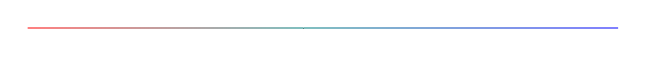
\begin{tikzpicture}
	\fill [left color=red!50, right color=teal!50] (0,0) rectangle (3.5,.01);
	\fill [left color=teal!50, right color=blue!50] (3.5,0) rectangle (7.5,.01);
	\end{tikzpicture}
\vspace{0.5cm}

$\boldsymbol \triangleright \ $ \textbf{Caso límite:} $\boldsymbol{\quad M\to \infty \ \Rightarrow \ \mu \to 0} \ \longrightarrow \ \begin{cases}
 \ \ddot X &=0 \\ \ \ddot x &= g \cos \theta \\ \ \ddot y &=g \cos^2 \theta - g =-g\sin^2 \theta	
 \end{cases}$ 
 
 Que coincide con los resultados que hubiésemos obtenido con mecánica newtoniana, como veremos al final del tema.
 
  \vspace{5mm}
  
\begin{myexampleblock}{Caso $M\to \infty$ con mecánica newtoniana}
 	
 	\begin{multicols}{2}
\begin{figure}[H]
	\centering
	\includegraphics[width=.45\textwidth]{imagenes/img10-02.png}
\end{figure}	
$\,$

$m$ se desplaza por el plano inclinado.

La componente $P_N$ se anula con la reacción $N$ del plano, solo queda la componentes $P_T=mg\sin \theta$. Solo hay movimieto en el eje $x'$.

Segunda de Newton: $º F_mg\sin \theta = ma$

Luego $a=g\sin \theta$

La proyección del vector $\vec a$ del eje $x`$ sobre los ejex $x$ e $y$ dan unas aceleraciones:
\end{multicols}
$a_x=\ddot x= g\sin \theta \cos \theta;\quad a_y=\ddot y= -g\sin^2 \theta\, , \ $ que coinciden con las que homos obtenido más arriba.
 \end{myexampleblock}
 
\vspace{1cm}
  

$\boldsymbol \triangleright \ $ \textbf{Caso límite:} $\quad \boldsymbol{\theta = 0}\, , \ $ la masa $m$ reposa sobre $M$.

Se obtiene, $\quad \ddot X=0;\quad \ddot x=0;\quad \ddot y=\dfrac{(1-\mu)g}{1-\mu}=g$, pero $\ \ddot y=0 \ $ al estar $m$ en el suelo.

\rule{200pt}{0.1pt}

Se cumplen perfectamente los casos límites.


 
 


